\section{Methods}

\begin{frame}[fragile=singleslide]{First and Follow}{}

\alert{First} and \alert{Follow} are functions defined over a grammar and they are used in \alert{parsing}

\begin{itemize}
    \item to distinguish two productions with the same non-terminal $X$ on the LHS, we examine the First($X$) sets for their corresponding RHS.
    \item set of terminal symbols that can follow a non-terminal $X$ in a parse as Follow(X).
\end{itemize}

\end{frame}

\note[itemize]{
\item First and Follow are functions used in parsing and they are recursively defined and we will use them to validate our implementation of the static evaluator.
}

\begin{frame}[fragile=singleslide]{Example}{Example of First and Follow}

\begin{multicols}{2}
\begin{Verbatim}[fontsize=\small]
S -> id
    | V assign E
V -> id
E -> V
    | num


First(S) = { id }
First(E) = { num, id }
First(V) = { id }

Follow(S) = { }
Follow(E) = { }
Follow(V) = { assign }
\end{Verbatim}
\end{multicols}

\end{frame}

\note[itemize]{
\item These are some examples of First and Follow.
}

\begin{frame}{Definition}{Formal recursive definition of First and Follow}

\[ \texttt{FIRST}(N) = \bigcup_{N \to \alpha} \texttt{FIRST}(\alpha) \]
\[ \texttt{FIRST}(\epsilon)   = \{ \epsilon \} \]
\[ \texttt{FIRST}(x \beta)   =\{x\} \]
\[ \texttt{FIRST}(N \beta)   =   \texttt{FIRST}(N) \cdot \texttt{FIRST}(\beta)  \]
\[ \texttt{FOLLOW}(N) = \bigcup_{N' \to \alpha N \beta} \texttt{FIRST}(\beta) \cdot \texttt{FOLLOW}(N') \]

\newlinevspace

Credit: Dr. Boyland's lecture notes
\end{frame}

\note[itemize]{
\item This a formal definition of First and Follow
\item Notice the recursive nature of the problem specifically in the last equation where we have Follow on both sides
}


\begin{frame}[fragile=singleslide]{Example}{Grammar definition in APS}

\begin{Verbatim}[fontsize=\tiny]
module GRAMMAR[] begin
  phylum Grammar;

  phylum Item;
  phylum Items := SEQUENCE[Item];

  phylum Production;
  phylum Productions := SEQUENCE[Production];

  constructor terminal(s: Symbol) : Item;
  constructor nonterminal(s: Symbol) : Item;
  constructor prod(nt: Symbol; children: Items) : Production;
  constructor grammar(prods: Productions) : Grammar;

  pragma root_phylum(type Grammar);
end;
\end{Verbatim}

\end{frame}

\note[itemize]{
\item This a definition of context-free grammar in APS
}

\begin{frame}[fragile=singleslide]{Example}{First implementation in APS}

\begin{Verbatim}[fontsize=\fontsize{2.5}{4}\selectfont]
module FIRST[T :: var GRAMMAR[]] extends T begin
  match ?self:Grammar=grammar(?prods: Productions) begin
    self.grammar_first := firstTable;
  end;
  
  match ?self:Production=prod(?nt:Symbol, ?items: Items) begin
    firstTable :> DeclarationTable$table_entry(nt, items.items_first);
  end;
  
  match ?self:Item=terminal(?s:Symbol) begin
    self.item_first := { s };
  end;
  
  match ?self:Item=nonterminal(?s:Symbol) begin
    case DeclarationTable$select(firstTable, s) begin
      match DeclarationTable$table_entry(?,?item_first_objs) begin
        self.item_first :> item_first_objs;
      end;
    end;
  end;
  
  match ?self : Items = Items$none() begin
    self.items_first :> { epsilon };
  end;
  
  match ?self : Items = Items$single(?item : Item) begin
    self.items_first :> item.item_first;
  end;
  
  match ?self : Items = Items$append(?items1,?items2 : Items) begin
    self.items_first := black_dot(items1.items_first, items2.items_first);
  end;
end;
\end{Verbatim}

\end{frame}
\note[itemize]{
\item This an implementation of First in APS
}


\begin{frame}[fragile=singleslide]{Example}{Follow implementation in APS}

\begin{Verbatim}[fontsize=\fontsize{2.5}{4}\selectfont]
module FOLLOW[T :: var GRAMMAR[]] extends T begin
  match ?self:Item=terminal(?s:Symbol) begin
    self.item_predict := { s };
  end;
  match ?self:Item=nonterminal(?s:Symbol) begin
    followTable :> DeclarationTable$table_entry(s, self.item_follow);
    case DeclarationTable$select(predictTable, s) begin
      match DeclarationTable$table_entry(?,?item_predict_objs) begin
        self.item_predict := item_predict_objs;
      end;
    end;
  end;
  match ?self:Production=prod(?nt:Symbol, ?items: Items) begin
    case DeclarationTable$select(followTable, nt) begin
      match DeclarationTable$table_entry(?,?item_follow_objs) begin
        items.items_follow := item_follow_objs;
      end;
    end;
    predictTable :> DeclarationTable$table_entry(nt, items.items_predict);
  end;
  match ?self:Grammar=grammar(?prods: Productions) begin
    self.grammar_follow := followTable;
  end;
  match ?self : Items = Items$none() begin
    self.items_predict := self.items_follow;
  end;
  match ?self : Items = Items$single(?item : Item) begin
    self.items_predict := item.item_predict;
    item.item_follow := self.items_follow;
  end;
  match ?self : Items = Items$append(?items1,?items2 : Items) begin
    items1.items_follow := items2.items_predict;
    items2.items_follow := self.items_follow;
    self.items_predict := items1.items_predict;
  end;
end;
\end{Verbatim}

\end{frame}

\note[itemize]{
\item This an implementation of Follow in APS
}


\begin{frame}{Fiber Construction}{Informal Definition: Beyond the scope of this presentation}

\small
\begin{itemize}
    \item A construction that expresses the semantics of \emph{remote attribute grammars} in \emph{classical terms}
    \item Objects implicitly carry separate values for the fields is like a \alert{rope} which can be separated into the individual fibers
    \item This yields an improper attribute grammar with an infinite number of attributes
    \item \emph{fiber approximation} fixes that (which then may include cycles ...)
\end{itemize}

\begin{center}
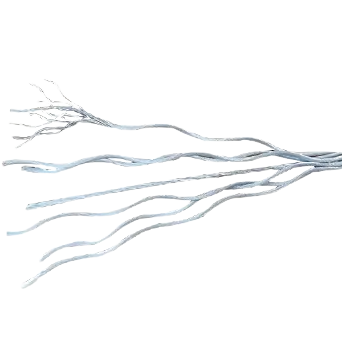
\includegraphics[scale=0.2]{rope-fiber.png}
\end{center}
    
\end{frame}

\note[itemize]{
    \item I am intentionally not going into details of fiber construction because it would be a disservice to remote attribute grammar paper
    \item Basically, its construction expresses the semantics of remote attribute grammars in classical terms
    \item Because objects implicitly carry separate values for the fields and it is like a rope that can be separated into the individual fibers
    \item But this yields an improper attribute grammar with an infinite number of attributes
    \item Then fiber approximation fixes that but it then may include cycles ...
}


\begin{frame}{Fiber Cycle Breaking}{Some fiber cycles are okay}

In RAG, some cycles can be ignored because they entirely involve so-called \alert{fiber attributes} that have no run-time significance. 

In CRAG, some cycles may carry value and will have run-time significance.
\end{frame}

\note[itemize]{
\item Even in a remote attribute grammar that is non-circular we may have fiber cycles and it's okay.
\item Fiber cycles are different between remote attribute grammar and circular remote attribute grammar because in the latter case, they may carry value. 
}



\begin{frame}{Fiber Cycle Breaking}{Issue with existing static scheduler}

Previously:
\begin{itemize}
    \item For every non-terminal whose fibered attributes take part in the cycle, created two \texttt{attribute\_decl} \alert{AST nodes} called up and down and connected all nodes to these to break cycles and preserve only UP followed by DOWN.
\end{itemize}

Now:

\begin{itemize}
    \item \alert{No creation of AST node}. Treat all nodes as either up or down. If the dependency is just fiber dependency then UP followed by DOWN. Otherwise, DOWN followed by UP.
\end{itemize}

\end{frame}

\note[itemize]{
\item Previous fiber cycle breaking module created two artificial attributes outside of the parser called UP and DOWN and this caused a lot of problems
\item To fix these we treat all attributes as either UP or DOWN and it simplified everything
}



\begin{frame}{Fiber Cycle Breaking}{Validated with RAG!}

\alert{Drop-in replacement} algorithm was successful.

\begin{itemize}
    \item Validated the algorithm against \alert{previous APS codes} that contained only fiber cycles and First and Follow APS codes
\end{itemize}

\end{frame}

\note[itemize]{
\item Tested the fiber cycle breaking algorithm against First and Follow the example.
\item And it was successful 
}



\begin{frame}{Static Scheduler}{Simplify scheduling by using groups}

Previously:
\begin{itemize}
    \item Old greedy scheduler was \alert{tightly coupled with code generation} module
\end{itemize}
    
Now:
\begin{itemize}
    \item Scheduling is still greedy but it is using groups and is simpler, easier to debug, and \alert{de-coupled from code generation} module.
    \item Includes $(\mathit{ph}, \mathit{ch})$ marker to help code generation identify the start and end of a child visit.
\end{itemize}

\end{frame}

\note[itemize]{
\item The static scheduler or the module that constructs the visit sequences was tightly coupled with the code generation module and it was not working well
\item So we designed a replacement that is still greedy but simpler as it schedules instances as groups and uses visit markers to indicate where child visit happens and when we need to return back to a parent visit from a child visit
}



\begin{frame}{Static Scheduler}{Validation in-progress ...}

\begin{itemize}
    \item Implementation is \alert{not finished yet}
\end{itemize}

\end{frame}

\note[itemize]{
\item The implementation of static schedule generation is currently in-progress but very close to being done.
}